\documentclass{../../../oss-apphys-exam}
\usepackage{enumitem}
\usetikzlibrary{decorations.markings}

\newcounter{last}

\begin{document}

\gentitle{2}{ELECTROSTATICS, PART 2}

\raggedcolumns

\runningheader{
  \fontfamily{phv}\small
  \textcolor{gray}{AP PHYSICS C: ELECTRICITY AND MAGNETISM $\blacksquare$}
  \textbf{MULTIPLE-CHOICE QUESTIONS}}{}{}


\begin{questions}
  \question Some electric field lines around two charges $A$ and $B$ are
  shown in the diagram below. Which of the following statement(s) are correct?
  \uplevel{
    \centering
    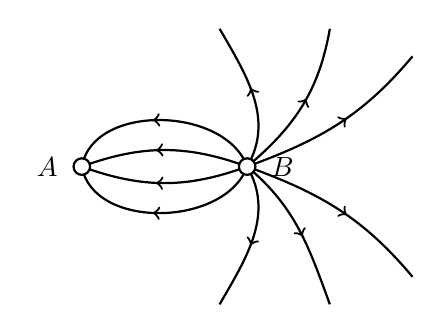
\begin{tikzpicture}[scale=.7,thick,decoration={
          markings,
          mark=at position 0.55 with {\arrow{>}}}
      ] 
      \draw[postaction={decorate}] (3,0) to[out=160,in=20] (0,0);
      \draw[postaction={decorate}] (3,0) to[out=200,in=-20] (0,0);
      
      \draw[postaction={decorate}] (3,0) to[out=110,in=80] (0,0);
      \draw[postaction={decorate}] (3,0) to[out=250,in=-80] (0,0);
      
      \draw[postaction={decorate}] (3,0) to[out=20,in=230] (6,2);
      \draw[postaction={decorate}] (3,0) to[out=-20,in=130] (6,-2);
      
      \draw[postaction={decorate}] (3,0) to[out=40,in=260] (4.5,2.5);
      \draw[postaction={decorate}] (3,0) to[out=-40,in=110] (4.5,-2.5);
      
      \draw[postaction={decorate}] (3,0) to[out=60,in=300] (2.5,2.5);
      \draw[postaction={decorate}] (3,0) to[out=-60,in=60] (2.5,-2.5);
      
      
      \draw[fill=white] circle (.15) node[left=5]{$A$};
      \draw[fill=white] (3,0) circle (.15) node[right=5]{$B$};
      
    \end{tikzpicture}
  }
  \begin{enumerate}[label=\Roman*.,nosep]
  \item Charge $A$ is positive
  \item The magnitude of charge $A$ is smaller than that of $B$.
  \item There is a neutral point to the right of $B$, where electric field
    is zero.
  \end{enumerate}
  \begin{choices}
    \choice I only
    \choice II only
    \choice I and III only
    \choice II and III only
    \choice None of the above statements are correct
  \end{choices}

  \question A small charged particle is projected in a uniform electric
  field. Which of the following trajectories is \textbf{impossible}?
  
  \begin{oneparchoices}
    \choice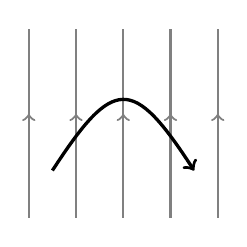
\begin{tikzpicture}[
      scale=.6,
      thick,
      decoration={
        markings,
        mark=at position 0.55 with {\arrow{>}}}
    ]
    \foreach \x in {0,...,4}
    \draw[gray,postaction={decorate}] (\x,0)--+(0,4);
    \draw[very thick,->] (.5,1) ..controls (1.8,3) and (2.2,3).. (3.5,1);
    \end{tikzpicture}
    
    \choice\begin{tikzpicture}[
      scale=.6,
      thick,
      decoration={
        markings,
        mark=at position 0.55 with {\arrow{>}}}
    ]
    \foreach \x in {0,...,4}
    \draw[gray,postaction={decorate}] (\x,0)--+(0,4);
    \draw[vectors] (.5,3.5) ..controls (1.8,0) and (2.2,0).. (3.5,3.5);
    \end{tikzpicture}
    \choice\begin{tikzpicture}[
      scale=.6,
      thick,
      decoration={
        markings,
        mark=at position 0.55 with {\arrow{>}}}
    ]
    \foreach \x in {0,...,4}
    \draw[gray,postaction={decorate}] (\x,0)--+(0,4);
    \draw[vectors] (1,3.5) ..controls (4,2.2) and (4,1.8).. (1,.5);
    \end{tikzpicture}
    
    \choice\begin{tikzpicture}[
      scale=.6,
      thick,
      decoration={
        markings,
        mark=at position 0.55 with {\arrow{>}}}
    ]
    \foreach \x in {0,...,4}
    \draw[gray,postaction={decorate}] (\x,0)--+(0,4);
    \draw[vectors] (.5,3.5) to[out=-65,in=180] (3.5,.5);
    \end{tikzpicture}
  \end{oneparchoices}
  
  \question A small object of mass $m$ and charge $q$ travels at an initial
  speed of \SI{100}{\metre\per\second} along the direction of a uniform
  electric field. After travelling over a distance of \SI{4}{\centi\metre},
  it is brought to a stop. What is the magnitude of the electric field?
  \begin{choices}
    \choice $\dfrac{5q}m$
    \choice $\dfrac{25q}m$
    \choice $\dfrac{25m}q$
    \choice $\dfrac{125q}m$
    \choice $\dfrac{125m}q$
  \end{choices}

  \question A beam of charged particles with the same velocity is directed
  into a gap between two parallel charged plates, where the electric field
  is uniform. All the particles follow the same path in the gap. Which of
  the following statements about the charged particles \textbf{must} be true?
  \begin{choices}
    \choice All of them have the same mass, but different charge
    \choice All of them have the same charge, but different mass
    \choice All of them have the same mass and charge
    \choice All of them have the same charge-to-mass ratio
  \end{choices}
  \newpage
  
  \question Electric potential
  \begin{choices}
    \choice is a vector quantity that depends on the direction of the electric
    field
    \choice is a scalar quantity that depends on the magnitude and sign of
    charges in the vicinity
    \choice is a scalar quantity that depends on the square of the distance
    from the charges in the vicinity
    \choice is a vector quantity that depends on the sign of the charges in
    the vicinity
    \choice is a vector quantity that must point from high to low potential
  \end{choices}

  \question A negative point charge $-Q$ is surrounded by eight positive
  point charges arranged along a circle, as shown in the figure below. The
  radius of the circle is $r$. How much work is required to bring the central
  charge to infinity?
  \uplevel{
    \centering
    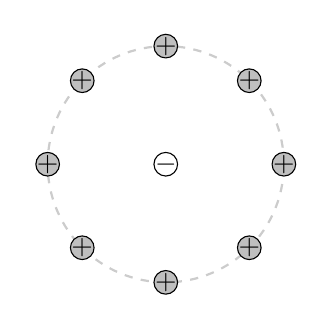
\begin{tikzpicture}
      \draw[thick,dashed,gray!40] circle (1.5);
      \foreach \theta in {0,45,...,350}
      \draw[rotate=\theta,fill=lightgray] (1.5,0) circle (.15) node{$+$};
      \draw circle (.15) node{$-$};
    \end{tikzpicture}
  }
  \begin{oneparchoices}
    \choice zero
    \choice $\dfrac{2Q^2}{\pi\varepsilon_0r}$
    \choice $\dfrac{2Q}{\pi\varepsilon_0r^2}$
    \choice $\dfrac{2Q^2}{\pi\varepsilon_0r}$
  \end{oneparchoices}
  
  \question A positively charged ring of radius $R$ is made of conducting
  material and has a charge $Q$ distributed uniformly around it. The center of
  the ring is located at point $0$ on the $x$-axis. The potential $V$ at a
  distance $3d$ from point $0$ on the $x$-axis is
  \begin{center}
    \begin{tikzpicture}
      \draw[ultra thick] ellipse (0.7 and 1.3);
      \draw[axes] (0,0)--(0,1.3) node[midway,right]{$R$};
      \draw[dashed] (0,0)--(0,-1.3);
      \draw[dashed] (-3.2,0)--(3.2,0);
      \foreach \x in {-3,-2,-1,1,2,3}
      \draw(\x,-.2)--(\x,.2) node[pos=0,below] {$\x d$};
    \end{tikzpicture}
  \end{center}
  \begin{choices}
    \choice $V=\dfrac{kQ}{9d^2}$
    \choice $V=\dfrac{kQ}{3d^2}$
    \choice $V=\dfrac{kQ}{R^2+9d^2}$
    \choice $V=\sqrt{\dfrac{kQ}{R^2+9d^2}}$
    \choice $V=\dfrac{kQ}{\sqrt{R^2+9d^2}}$
  \end{choices}
    
  \question Which of the following statements is true of electric field and
  equipotential lines?
  \begin{choices}
    \choice The electric field vector always points in the same direction as
    the equipotential lines.
    \choice The electric field always points in the opposite direction of the
    equipotential lines.
    \choice The electric field always points perpendicular to the
    equipotential lines.
    \choice The electric field is always equal to the equipotential lines.
    \choice Equipotential lines always form a circle around electric field
    lines.
  \end{choices}
  \newpage
  
  \question The potential $V$ as a function of distance $r$ for a particular
  charge distribution is given by the equation $V=ar^{-1}$. The electric field
  as a function of distance $r$ from the charge distribution is
  \begin{choices}
    \choice $\dfrac13ar^{-3}$
    \choice $2ar^{-1}$
    \choice $ar^{-2}$
    \choice $-a(\ln r)$
    \choice $-ar^{-2}$
  \end{choices}
\end{questions}
\setcounter{last}{\value{question}}
\newpage

\runningheader{
  \fontfamily{phv}\small
  \textcolor{gray}{AP PHYSICS C: ELECTRICITY AND MAGNETISM $\blacksquare$}
  \textbf{FREE-RESPONSE QUESTIONS}}{}{}


% TAKEN FROM 2010 AP PHYSICS C EXAM FREE-RESPONSE QUESTION E&M 1
% MODIFIED FROM THE STANDARD QUESTION
\begin{center}
  \begin{tikzpicture}[scale=1.2]
    \draw[axes] (-2,0)--(2,0) node[right]{$x$};
    \draw[axes] (0,-2)--(0,2) node[above]{$y$};
    \draw[gray] circle (1.3);
    \begin{scope}[rotate=135]
      \draw[line width=3] (1.3,0) arc (0:90:1.3) node[pos=.3,left]{$+Q$};
      \draw[axes,dashed] (0,0)--(1.3,0) node[pos=.65,below]{$R$};
    \end{scope}
    \fill[rotate=45] (1.3,0) circle(.055) node[above right]{$A$};
    \fill[rotate=-45](1.3,0) circle(.055) node[below right]{$C$};
    \fill (.6,0) circle (.055) node[above]{$B$};
  \end{tikzpicture}
\end{center}

\begin{questions}
  \setcounter{question}{\value{last}}
  
  \question A charge $+Q$ is uniformly distributed over a quarter circle of
  radius $R$, as shown above. Points $A$, $B$, and $C$ are located as shown,
  with $A$ and $C$ located symmetrically relative to the $x$-axis. Express all
  algebraic answers in terms of the given quantities and fundamental constants.
  \begin{parts}
    \part\textbf{Rank} the magnitude of the electric potential at points $A$,
    $B$, and $C$ from greatest to least, with number 1 being greatest. If two
    points have the same potential, give them the same ranking.

    \vspace{.1in}
    \underline{\hspace{.3in} } $V_A$ \hspace{.3in}
    \underline{\hspace{.3in} } $V_B$ \hspace{.3in}
    \underline{\hspace{.3in} } $V_C$

    \vspace{.1in}\textbf{Justify} your rankings.
    \vspace{\stretch1}
    
    \uplevel{
      Point $P$ is at the origin, as shown below, and is the centre of
      curvature of the charge distribution.
      \begin{center}
        \begin{tikzpicture}[scale=1.2]
          \draw[axes] (-2,0)--(2,0) node[right]{$x$};
          \draw[axes] (0,-2)--(0,2) node[above]{$y$};
          \draw[gray] circle (1.3);
          \begin{scope}[rotate=135]
            \draw[line width=3] (1.3,0) arc (0:90:1.3) node[pos=.3,left]{$+Q$};
            \draw[axes,dashed] (0,0)--(1.3,0) node[pos=.65,below]{$R$};
          \end{scope}
          \fill circle(.055) node[below right]{$P$};
        \end{tikzpicture}
      \end{center}
    }

    \part\textbf{Determine} an expression for the electric potential at point
    $P$ due to the charge $Q$.
    \vspace{\stretch1}
    \newpage
    
    \part A positive point charge $q$ with mass $m$ is placed at point $P$ and
    released from rest. \textbf{Derive} an expression for the speed of the
    point charge when it is very far from the origin.    
    \vspace{\stretch1}
    
    \part On the dot representing point $P$ below, \textbf{indicate} the
    direction of the electric field at point $P$ due to the charge $Q$.
    \begin{center}
      \begin{tikzpicture}[axes]
        \draw (-2,0)--(2,0) node[right]{$x$};
        \draw (0,-2)--(0,2) node[above]{$y$};
        \fill circle (.08);
      \end{tikzpicture}
    \end{center}
    
    \part\textbf{Derive} an expression for the magnitude of the electric field
    at point $P$.
    \vspace{\stretch2}
  \end{parts}
  \newpage


  
  % TAKEN FROM 2016 AP PHYSICS C EXAM FREE-RESPONSE QUESTION E&M 1
  \uplevel{
    \cpic{.9}{potentials}
  }
  \question Two point charges, $q_1$ and $q_2$, are fixed in place on the
  $x$-axis at positions $x_1=\SI{-1.00}\metre$ and $x_1=+\SI{.50}\metre$,
  respectively. Charge $q_2$ has a value of \SI{2.0}{\nano\coulomb}. Values of
  electric potential are illustrated by the given equipotentials in the diagram
  shown above, which is drawn to scale.
  \begin{parts}
    \part\textbf{Calculate} the value of $q_1$.
    \vspace{\stretch1}
    
    \part At point $C$ on the diagram, \textbf{draw} a vector representing the
    direction of the electric field at that point.
    
    \part\textbf{Calculate} the approximate magnitude of the electric field
    strength at point $D$ on the diagram.
    \vspace{\stretch1}
    
    %\part The equipotential labeled $\SI0\volt$ is the cross section of a
    %nearly spherical surface. Calculate the electric flux for this surface.
    %\vspace{\stretch1}
    \newpage
    
    \uplevel{
      A proton is placed at point $A$ and then released from rest.
    }
    
    \part\textbf{Calculate} the work done by the electric field on the proton
    as it moves from point $A$ to point $E$.
    \vspace{\stretch1}
      
    \part\textbf{Calculate} the speed of the proton when it reaches point $E$.
    \vspace{\stretch1}
    
    \part An electron is released from rest at point $B$. \textbf{Indicate} the
    direction of the initial acceleration, if any, of the electron?

    \vspace{.1in}
    \underline{\hspace{.3in}} Up\hspace{.2in}
    \underline{\hspace{.3in}} Down\hspace{.2in}
    \underline{\hspace{.3in}} Left\hspace{.2in}
    \underline{\hspace{.3in}} Right\hspace{.2in}
    \underline{\hspace{.3in}} Into the page\hspace{.2in}
    \underline{\hspace{.3in}} Out of the page

    \vspace{.1in}\underline{\hspace{.3in}} The direction is undefined since the
    acceleration is zero.

    \vspace{.1in}\textbf{Justify} your answer.
    \vspace{\stretch3}
    
  \end{parts}
  \newpage
  
  \question A spherically symmetric charge distribution has net positive charge
  $Q_0$ distributed within a radius of $R$. Its electric potential $V$ as a
  function of the distance $r$ from the center of the sphere is given by the
  following
  \begin{align*}
    V(r) &= \frac{Q_0}{4\pi\epsilon_0R}\left[-2+3\left(\frac rR\right)^2 \right]
    \text{ for } r<R\\
    V(r) &= \frac{Q_0}{4\pi\epsilon_0r}\text{ for } r>R
  \end{align*}
  Express all algebraic answers in terms of the given quantities and
  fundamental constants.
  \begin{parts}
    \part For the following regions, \textbf{indicate the direction} of the
    electric field $E(r)$ and \textbf{derive} an expression for its magnitude.
    \begin{subparts}
      \subpart $r < R$
      
      \vspace{.1in}\underline{\hspace{.4in}} Radially inward
        
      \vspace{.1in}\underline{\hspace{.4in}} Radially outward
      \vspace{\stretch1}
      
      \subpart $r > R$
      
      \vspace{.1in}\underline{\hspace{.4in}} Radially inward

      \vspace{.1in}\underline{\hspace{.4in}} Radially outward
      \vspace{\stretch1}
      
    \end{subparts}
    
    \part For the following regions, \textbf{derive} an expression for the
    enclosed charge that generates the electric field in that region, expressed
    as a function of $r$.
    \begin{subparts}
      \subpart $r < R$
      \subpart $r > R$
    \end{subparts}
    \vspace{\stretch1}
    \newpage
    
    \part\textbf{Indicate} whether there is any charge on the surface of the
    sphere ($r=R$).

    \vspace{.1in}
    \underline{\hspace{.4in}} Yes\hspace{.3in}
    \underline{\hspace{.4in}} No
    
    If there is, \textbf{determine} the charge. In either case,
    \textbf{explain} your reasoning.
    \vspace{\stretch1}
    
    \part On the axes below, \textbf{sketch} a graph of the force that would
    act on a positive test charge in the regions $r<R$ and $r > R$. Assume that
    a force directed radially outward is positive.
    \begin{center}
      \begin{tikzpicture}[scale=1.1]
        \draw[axes] (0,-3)--(0,3) node[above]{$F$};
        \draw[axes] (0,0)--(10,0) node[right]{$r$};
        \draw[dashed] (4,-3)--(4,3) node[midway,below left]{$R$};
      \end{tikzpicture}
    \end{center}
  \end{parts}
  \vspace{\stretch1}
\end{questions}
\end{document}
